\begin{frame}[t]{Set union keeps shared observations once; mutual information describes dependence.\ev{\tagA}}
\begin{center}
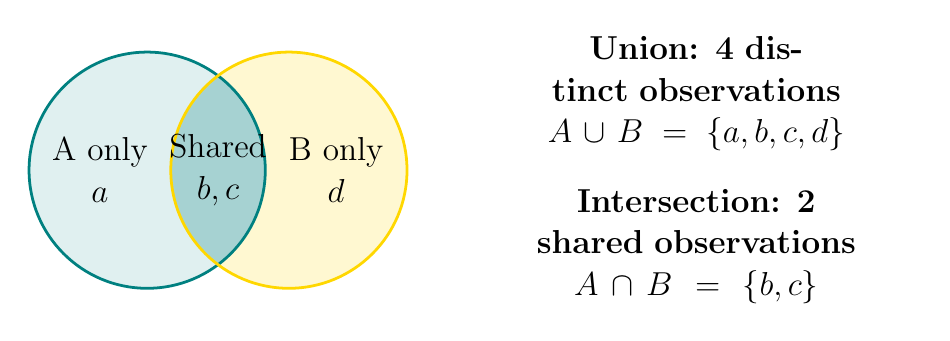
\begin{tikzpicture}[x=1cm,y=1cm,every node/.style={align=center,font=\fontsize{12}{15}\selectfont}]
\fill[Teal!12](-.9,0)circle(1.5);\fill[Gold!18](.9,0)circle(1.5);
\begin{scope}\clip(-.9,0)circle(1.5);\fill[Teal!35](.9,0)circle(1.5);\end{scope}
\draw[Teal,line width=1pt](-.9,0)circle(1.5);\draw[Gold,line width=1pt](.9,0)circle(1.5);
\node at(-1.5,0){A only\\$a$};\node at(0,0){Shared\\$b,c$};\node at(1.5,0){B only\\$d$};
\node[anchor=west,text width=5.5cm]at(3.2,0){\textbf{Union: 4 distinct observations}\\$A\cup B=\{a,b,c,d\}$\\[10pt]\textbf{Intersection: 2 shared observations}\\$A\cap B=\{b,c\}$};
\end{tikzpicture}
\end{center}
\tagline{Entropy $H$: uncertainty. Mutual information $I$: dependence.\\For random variables: $H(X,Y)=H(X)+H(Y)-I(X;Y)$.}
\sources{Set diagram: exact illustrative observation IDs. Entropy identity: \href{https://ocw.mit.edu/courses/6-441-information-theory-spring-2016/pages/lecture-notes/}{MIT information-theory notes}.}
\qadetail{The circles show overlap of observed-item sets, not areas proportional to Shannon entropy. Cardinality inclusion-exclusion counts each declared observation once. For discrete random variables the joint-entropy identity subtracts their mutual information from the sum of marginal entropies. This is not a prescription to subtract pairwise mutual information from Fisher information or from precision. Entropy of observations differs from information about a parameter. Pairwise dependence need not determine higher-order dependence. Target information can be expressed by the chain rule I(theta;X,Y)=I(theta;X)+I(theta;Y|X), where the second term is the extra information about theta after observing X. The covariance-based example later uses unbiased same-parameter estimates with externally known positive-definite error covariance. Dependence beyond that model needs a justified joint model or conservative uncertainty treatment.}
\note{[0:45] Branch A used observations a, b and c. Branch B used b, c and d. Collecting the union gives four distinct observations, because b and c were shared. This is exact duplicate accounting. Different observations can also be statistically dependent. Mutual information measures that dependence, and the entropy identity expresses shared uncertainty. It does not by itself tell us how to weight estimates of a target. For that, we need a statistical model. The useful question is what extra information branch B adds after we have already seen branch A.}
\end{frame}
